\documentclass[times, utf8, diplomski]{fer}
\usepackage{booktabs}
\usepackage{subcaption}
\usepackage{amsmath}
\usepackage{pythonhighlight}
\usepackage{xcolor}
\usepackage{listings}
\usepackage{minted}
\usepackage{algorithm2e}

% Promjeni listing caption
\renewcommand{\listingscaption}{Izvorni kod}

\begin{document}

% TODO: Navedite broj rada.
\thesisnumber{1935}

% TODO: Navedite naslov rada.
\title{Lokalizacija autonomnog vozila u simuliranom urbanom okruženju}

% TODO: Navedite vaše ime i prezime.
\author{Matija Vukić}

\maketitle

% Ispis stranice s napomenom o umetanju izvornika rada. Uklonite naredbu \izvornik ako želite izbaciti tu stranicu.
%\izvornik
\begin{center}
  \makebox[\textwidth]{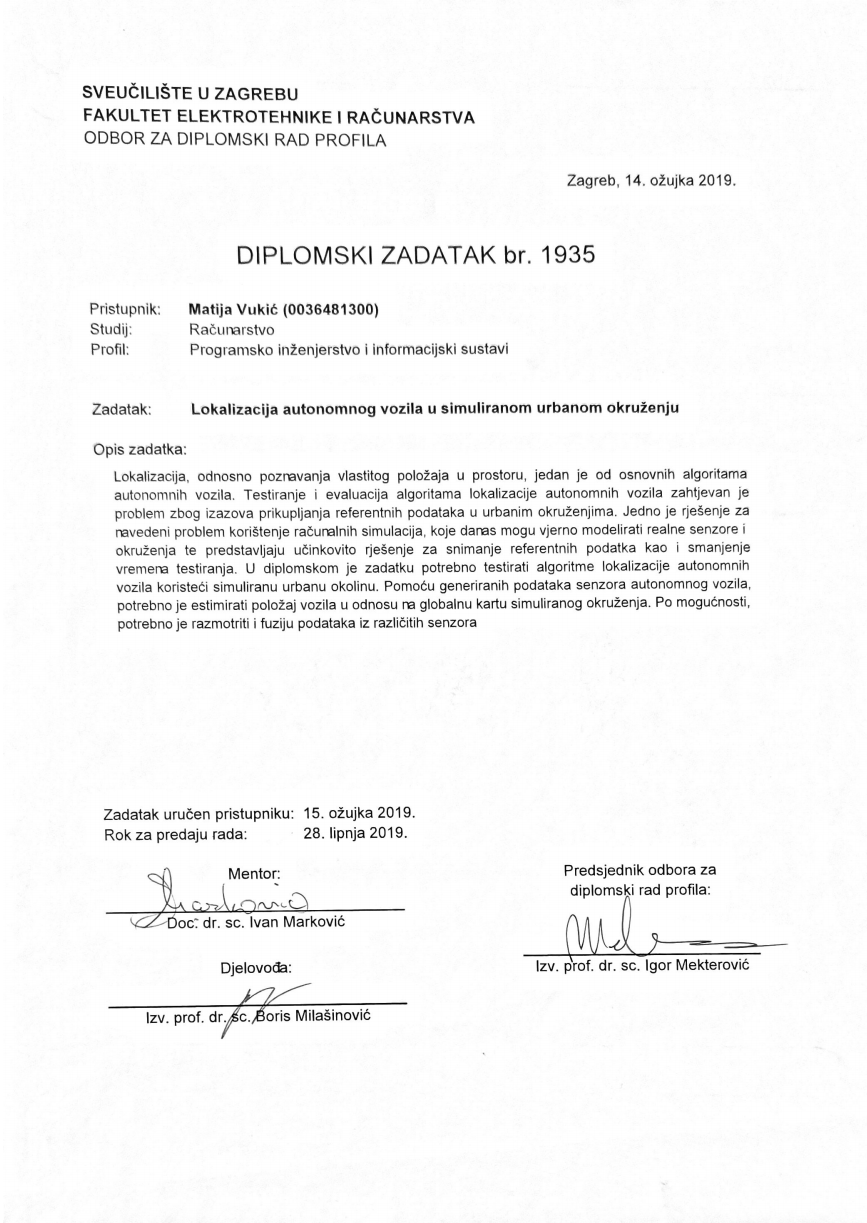
\includegraphics[width=\paperwidth]{images/izvornik.png}}
\end{center}

% Dodavanje zahvale ili prazne stranice. Ako ne želite dodati zahvalu, naredbu ostavite radi prazne stranice.
\zahvala{Zahvala mentoru Doc. Dr. Sc. Ivanu Markoviću za strpljenje i vodstvu}

\tableofcontents
\chapter{Uvod}
Uvod rada. Nakon uvoda dolaze poglavlja u kojima se obrađuje tema. %ok

\chapter{Problem lokalizacije vozila}
\section{Lokalizacija}

Lokalizacija je ... %ok
\section{Problem lokalizacije}

Problem lokalizacije je netočnost algoritama i šum u očitanjima. %ok

\chapter{Priprema podataka}
\section{Simulator}

Za točne referentne podatke potrebno je imati simulirano okruženje. Takvo simulirano okruženje se zove simulator. Potreban je simulator koji već ima integrirane razne mape, razne senzore, vozila te način komunikacije s tim vozilima iz vanjskih skripti. Neki od simulatora su opisani u sljedećem tekstu.

\subsubsection{Carla}
\begin{figure}[ht!]
  \centering
  
\includegraphics[scale=0.5]{images/carla_logo.png}
  \caption{Carla logo\cite{logo:carla}}
\end{figure}

Carla\cite{dosovitskiy17} je simulacijsko okruženje koje služi za testiranje metoda i algoritama prilikom razvoja autonomnih vozila. U pozadini koristi Unreal Engine za izvršavanje simulacije. Simulator se ponaša kao poslužitelj koji prima naredbe iz vanjskih klijentskih programa. Ti klijentski programi su pisani u programskom jeziku pytohn.
Carla ima integirane razne senzore te su neki od njih RGB kamera, Lidar senzor, senzor dubine, GNSS, ... Sponzori projekta su Intel, Toyota, GM i Computer vision Center. Više o ovome simulatoru će biti u sljedećem poglavlju.
\pagebreak
\subsubsection{Apollo}
\begin{figure}[ht!]
  \centering
  
\includegraphics[scale=0.2]{images/apollo_logo.png}
  \caption{Apollo logo\cite{logo:apollo}}
\end{figure}

Apollo je također rješenje za testiranje autonomnoh vozila. Sadrži simulator ali također je i potpuno komercijalno rješenje. Podržava razne scenarije, ima sustav ocjenjivanja koji daje ocjenu na temelju desetak metrika. Simulacije zapravo provodi u oblaku tj. koristi Microsoft Azure. Sponzori projekta su mnoge azijske tvrtke kao i Ford, Microsoft, Daimler, Honda, Intel i ostali.

\subsubsection{rFpro}
\begin{figure}[ht!]
  \centering
  
\includegraphics[scale=0.2]{images/rfpro_logo.jpg}
  \caption{rFpro logo\cite{logo:rfpro}}
\end{figure}

rFpro je kompletno rješenje za testiranje autonomnih vozila. U potpunosti je kommercijalno rješenje ali je zato jedno od najboljih u svijetu. Uglavnom je usredotočeno na primjenu strojnog učenja u autonomnim vozilima. Ima jednu od najvećih baza digitaliziranih stvarnih likacija diljem svijeta. Dinamički sustav vremena omogućuje testiranje ponašanja vozila u raznim vremenskim uvjetima. Sponzori projekta su BMW, Shell, GM, Renault i ostali.
\pagebreak
\subsubsection{AVSimulation}
\begin{figure}[ht!]
  \centering
  
\includegraphics{images/avsimulation_logo.png}
  \caption{AVSimulation logo\cite{logo:avsimulation}}
\end{figure}

AVSimulation se zapravo sastoji od simulatora vožnje i samog simulatora SCANeR. SCANeR je skup aplikacija koji pružaju rute, senzore, vozila, dinamičko vrijeme, pisanje skripti. Vrlo je modularan. Smulator vožnje je zapravo kupola koja se sastoji od cijelog vozila te se zapravo kretanje tog vozila simulira unutar te kupole. Sponzori su Renault, PSA, Volvo, Microsoft, Mazda i ostali.
\newpage %ok
\section{Opis okruženja}

Simulacijsko okruženje će biti Carla zato što ima vrlo široko programsko sučelje za upravljanje aspektima simulacije te je besplatno za korištenje. Simulator se pokreće kao poslužitelj te se vozila dodaju pomoću skripte koja je napisana u programskom jeziku python.

\begin{figure}[ht!]
  \centering
  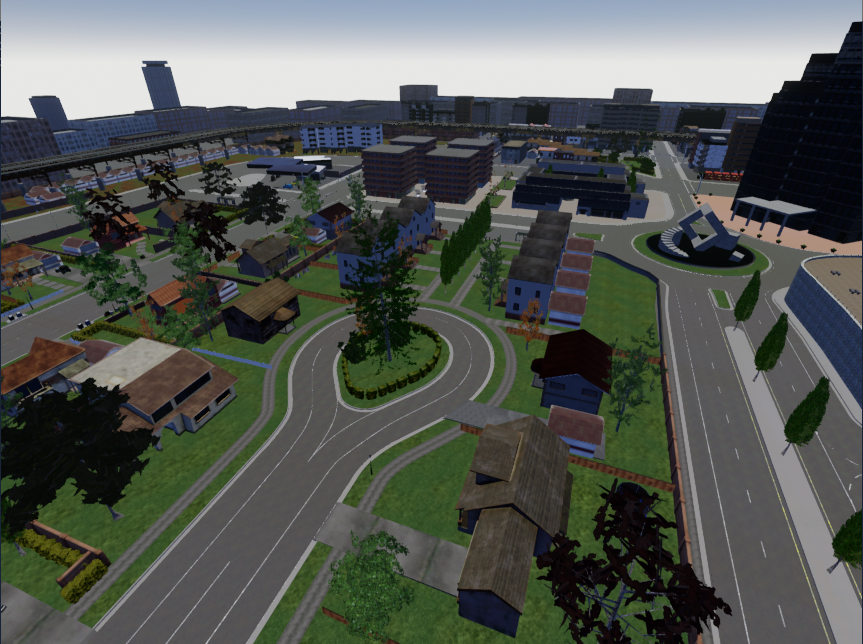
\includegraphics[scale=0.5]{images/carla_town03_example.png}
  \caption{Primjer karte pod nazivom Town03}
  \label{fig:town03_exmaple}
\end{figure}

Na slici \ref{fig:town03_exmaple} se vidi pogled na jedan od 7 mapa iz perspektive slobodne kamere. Korištene mape su definirane OpenDrive standardom. Simulator podržava raznolike senzore. Svi ti senzori se mogu postaviti samostalno na mapu, ali su najkorisniji kada se postave na drugo vozilo.

\newpage
\subsection{Senzori}
\subsubsection{RGB senzor}
\begin{figure}[ht!]
  \centering
  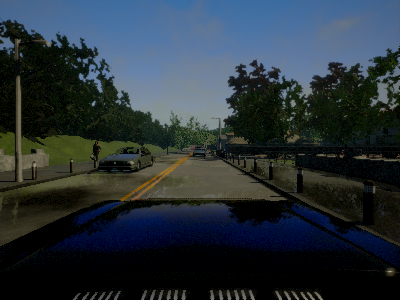
\includegraphics[scale=0.5]{images/rgb_example.png}
  \caption{Primjer regularne kamere\cite{carla:sensors}}
  \label{fig:rgb_exmaple}
\end{figure}

RGB senzor simulira kameru koja može snimati sliku koristeću crvenu, zelenu i plavu boju, tj. regularnu kameru. Ovaj senzor može prikupljati podatke iz simulatora u video obliku ili kao niz slika. Ovaj senzor se može koristiti u metodama lokalizacije koje kao temeljni algoritam koriste prepoznavanje ostalih sudionika u prometu prema obliku tj algoritmi prepoznavaju kontekst slike.

\subsubsection{Senzor dubine}
\begin{figure}[ht!]
  \centering
  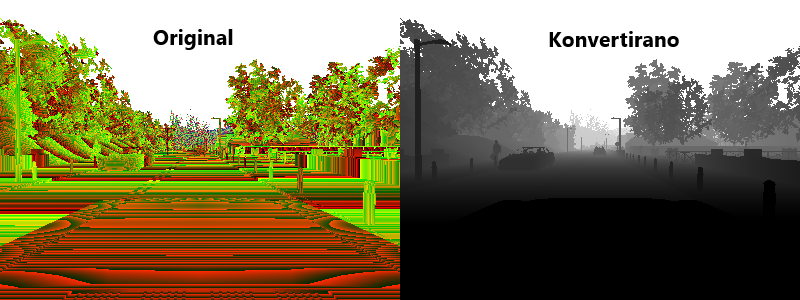
\includegraphics[scale=0.5]{images/depth_example.png}
  \caption{Primjer rezultata senzora dubine\cite{carla:sensors}}
  \label{fig:depth_exmaple}
\end{figure}

Ovaj senzor koristi nizove projicirajućih točaka da bi ilustrirao udaljenosti objekata, original na slici \ref{fig:depth_exmaple}. Tada se ti podaci pretvaraju u crno bijelu sliku gdje je svaki pixel u nijansama sive boje tj. ovisno koliko je objekt na određnome pixelu odaljen od kamere imati će svijetliju nijansu, konvertirano na slici \ref{fig:depth_exmaple}.

\newpage
\subsubsection{Semantičke segmentacije}
\begin{figure}[ht!]
  \centering
  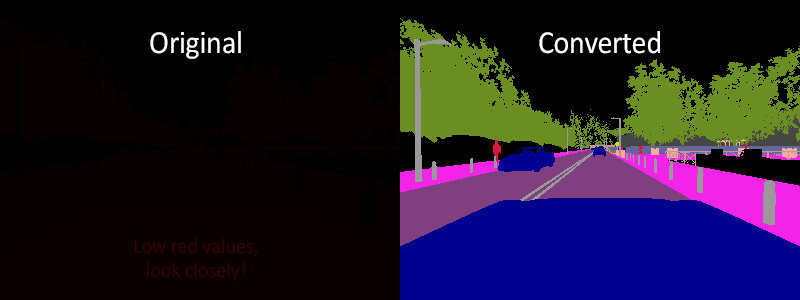
\includegraphics[scale=0.5]{images/sem_seg_exmaple.png}
  \caption{Primjer semantičke segmentacija\cite{carla:sensors}}
  \label{fig:sem_seg_exmaple}
\end{figure}

Ovaj senzor zapravo nije senzor ali je grupiran u klasu senzora zato što radi na vrlo sličan način kao i ostali senzori u simulatoru. Ovaj senzor dijeli sliku kamere na semantičke dijelove tj. objekte različitog tipa predstavlja drugim bojama. Na slici \ref{fig:sem_seg_exmaple} se vidi da je nebo crne boje, auti su plave boje, drveće je zeleno itd. OVaj način raspoznavanja objekata je moguć samo u simulator zato što nije potrebno razpoznavati objekte na slici već su oni definirani u simuliranoj okolini.

\subsubsection{LIDAR senzor}
\begin{figure}[ht!]
  \centering
  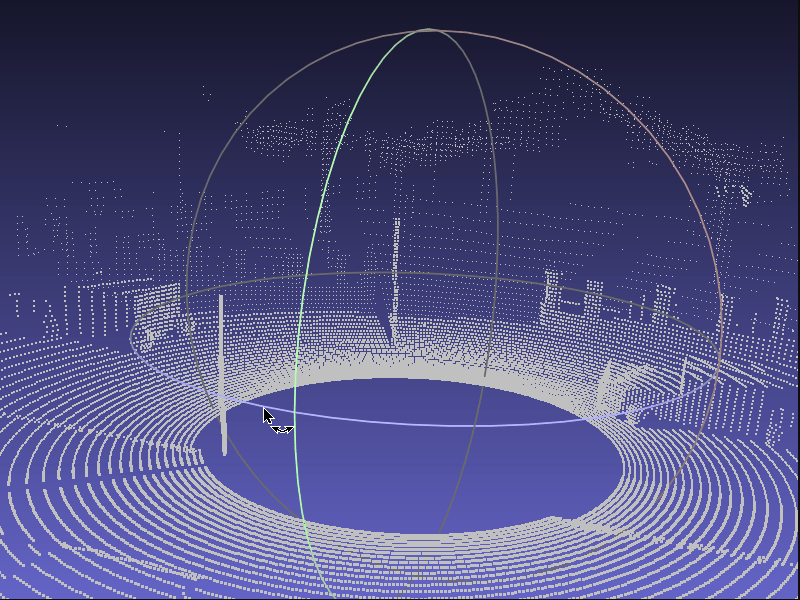
\includegraphics[scale=0.5]{images/LIDAR_examaple.png}
  \caption{LIDAR podaci\cite{carla:sensors}}
  \label{fig:lidar_exmaple}
\end{figure}
LIDAR (eng. light detecting and raging) senzor je zapravo vertikalan skup lasera koji simuliraju skeniranje od 360 stupnjeva tako da se rotiraju određeni broj puta u sekundi. Povratni podaci senzora su zapravo točke tj. koordinate relativne naspram samoga senzora do kojih su laseri uspjeli doći. Na slici \ref{fig:lidar_exmaple} se mogu vidjeti takvi podaci vizualizirani u programu MeshLab. Više o ulaznim parametrima senzora kasnije u radu.

\subsubsection{Senzor sudara}
Ovaj senzor dojavljuje klijentskome programu ako se vozila sudarilo s drugim objektom u simulaciji.

\subsubsection{Senzor prijelaza trake}
Ovaj senzor dojavljuje klijentskome programu ako je vozilo prošlo preko trake na cesti.

\subsubsection{GNSS senzor}
Senzor koji dojavljuje klijentskome programu trenutnu GNSS lokaciju vozila. Ta lokacija se interno računa tako da se lokacija vozila dodaje na geografsku referentnu lokaciju definiranu za cijelu mapu.

\subsubsection{Senzor prepreke}
Ovaj senzor javlja klijentskome programu ako se ispred vozila nalazi prepreka.

\subsection{Promet}
Postoji poveći broj već unaprijed definiranih vozila koja se mogu koristiti. Mogu se koristiti kao nositelji senzora ili kao ostali sudionici u prometu. Carla ima dobro definirana prometna pravila te semafore da bi simulacija izgledala što vjernije.
\newpage %ok
\section{Point cloud}

Oblak točaka ili skup točaka (eng. point cloud) je nakupina točaka u trodimenzionalnom koordinatnome sustavu. %ok
\section{Referentni podaci}

Referentni podaci su oni podaci s kojima se uspoređuju rezultati metoda. Ti referentni podaci su generirani u simulatoru te predstavljaju lokaciju i rotaciju vozila u jednome trenutku. Referentni podaci se zapravo sastoje od lokacije i rotacije vozila.

\subsubsection{Lokacija}
Lokacija vozila je također definirana kao točka u kartezijevom koordinatnome prostoru. Sastoji se od x, y i z koordinata. Slično kao prikazano na slici \ref{fig:point_coordinates}.


\subsubsection{Rotacija}
 U trodimenzialnome prostoru objekt se zapravo može rotirati oko beskonaćnoga broja osi ali se u pravilu uzimaju 3 statičke osi. Te osi se nazivaju os skretanja (eng. yaw), os poniranja (eng. pitch) i os valjanja (eng. roll). 

\begin{figure}[!ht]
  \centering
  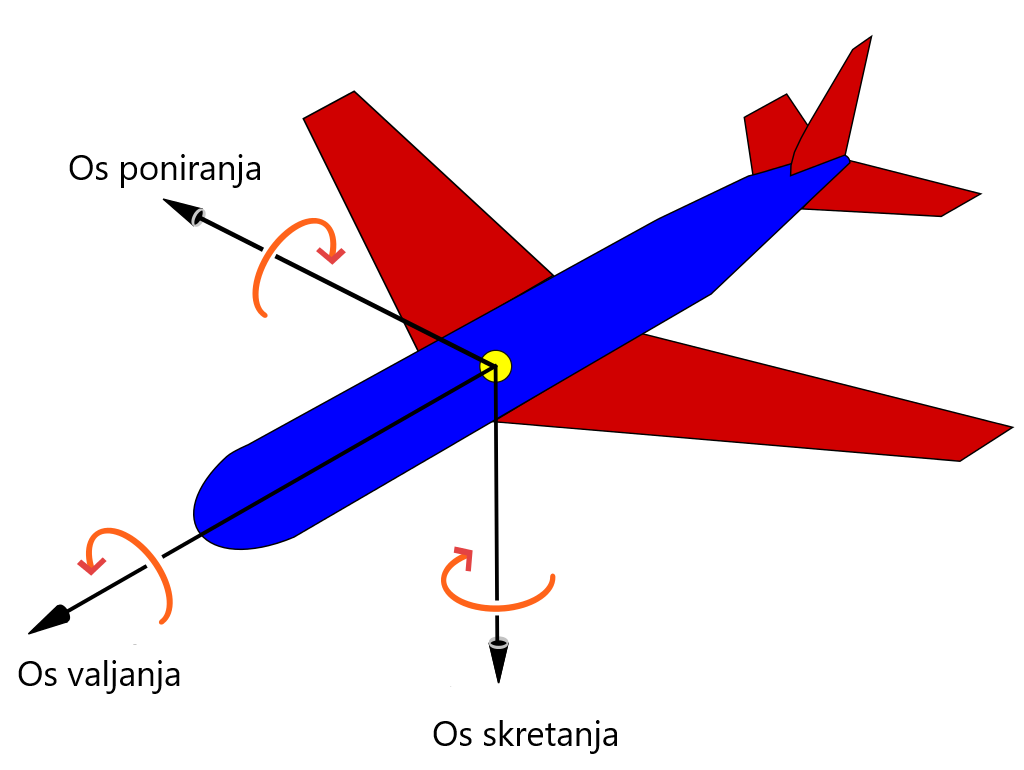
\includegraphics[scale=0.3]{images/yaw_roll_pitch_example.png}
  \caption{Ilustracija osi rotiranja}
  \label{fig:yaw_roll_pitch_example}
\end{figure}


Os rotacije je os koja prolazi u smjeru kretanja vozila (x os), os poniranja je zapravo os okomita s os rotacija (z os), dok je os skretanja okomita na obje prethodne osi (y os). Te osi su ilustrirane na slici \ref{fig:yaw_roll_pitch_example}.

Vizualizacije referentnih podataka za jedan primjer kretanja vozila možemo vidjeti na sljedećim slikama. Na svim grafovima svaka točka predstavlja jedno očitanje. Grafovi su izgrađeni pomoću programskog jezika Kotlin koristeći biblioteku XChart. Slika \ref{fig:gt_lokacija} prikazuje graf lokacija vozila. Slika \ref{fig:gt_lokacija_x} pokazuje x koordinate vozila  uvremenu. Slika \ref{fig:gt_lokacija_y} pokazuje y koordinate vozila u vremenu. Slika \ref{fig:gt_rotacija} pokazuje vrijednosti rotacija oko statičkih osi u vremenu. Za očekivati je kako će se mjenjati samo rotacija skretanja zato što vozilo može skretati, a ne može ponirati ili se valjati. 

\begin{figure}[h!]
  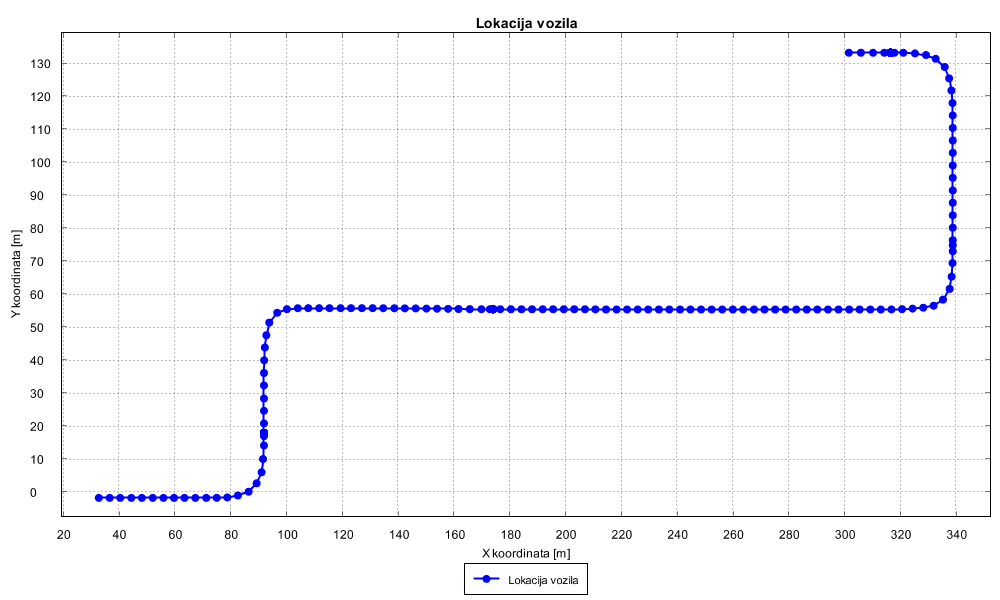
\includegraphics[scale=0.4]{images/gt_lokacija.png}
  \caption{Graf lokacije vozila}
  \label{fig:gt_lokacija}
\end{figure}
\pagebreak
\begin{figure}[h!]
  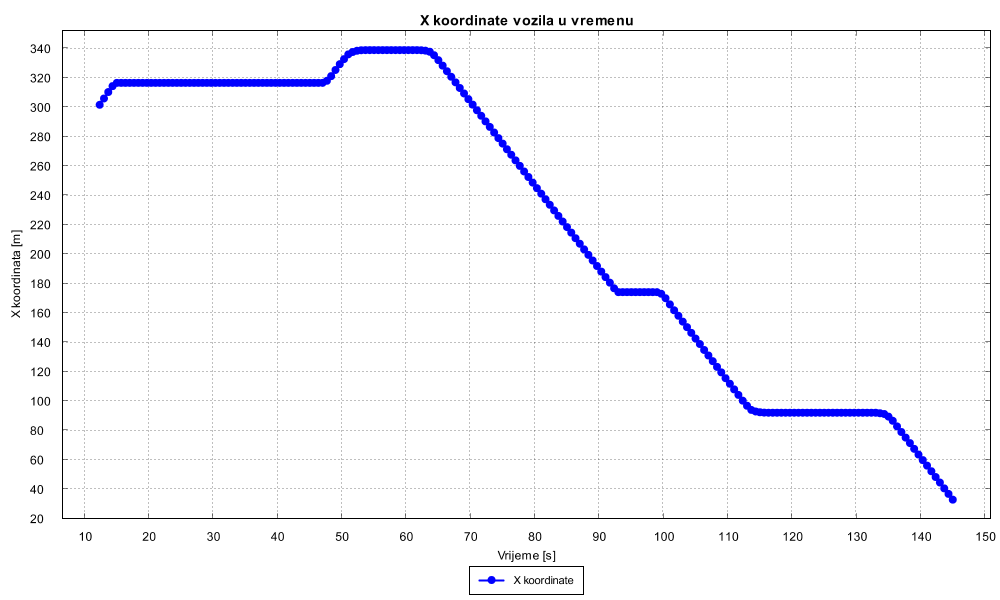
\includegraphics[scale=0.4]{images/gt_lokacija_x.png}
  \caption{Graf X lokacije vozila u vremenu}
  \label{fig:gt_lokacija_x}
\end{figure}
\begin{figure}[h!]
  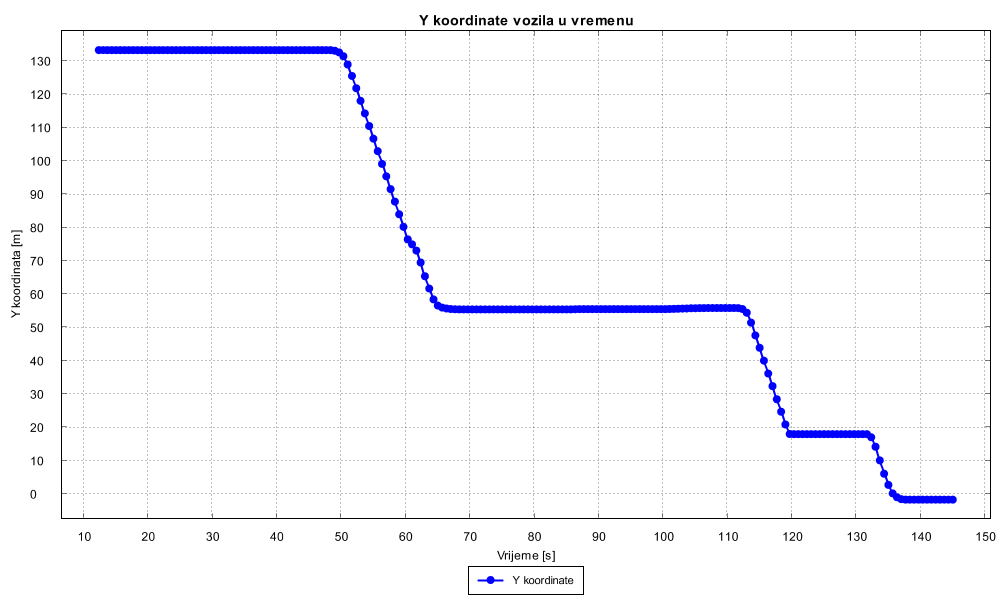
\includegraphics[scale=0.4]{images/gt_lokacija_y.png}
  \caption{Graf Y lokacije vozila u vremenu}
  \label{fig:gt_lokacija_y}
\end{figure}
\pagebreak
\begin{figure}[h!]
  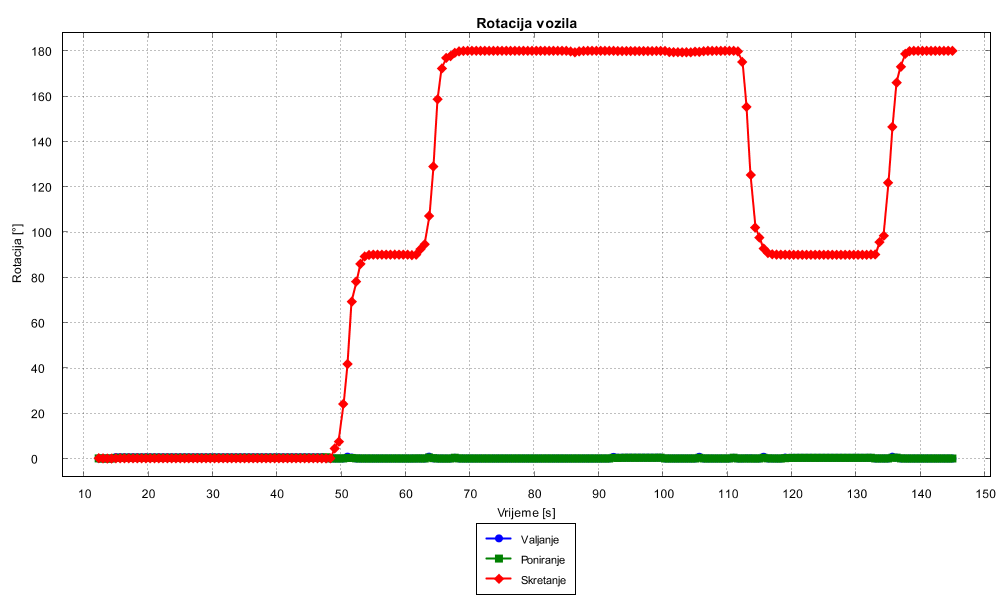
\includegraphics[scale=0.4]{images/gt_rotacija.png}
  \caption{Graf rotacija u vremenu}
  \label{fig:gt_rotacija}
\end{figure} %ok
\section{Izvor podataka}
Kao izvor podataka za algoritme se koristi već prije spomenuti LIDAR senzor. S obzirom da je senzor simuliran, možemo mu postavljati sljedeće parametre:

\begin{itemize}
  \item Broj kanala - broj lasera
  \item Donja granica polja vida - koliko nisko su orijentirani laseri
  \item Gornja granica polja vida - koliko visoko su orijentirani laseri
  \item Ukupan broj točaka - ukupan broj točaka po laseru u očitanju
  \item Frekvencija rotacije - koliko četo se laseri rotiraju
  \item Vremenski korak - koliko često se podaci očitavaju
\end{itemize}

Podaci koje nam vrati senzor su zapravo u obliku skupa točaka (eng. Point Cloud). %ok
\pagebreak
\section{Prikupljanje podataka}

Podaci su prikupljeni tako da se simulator pokrene u poslužiteljkom načinu rada te se tada pokreće klijentska skripta napisana u python jeziku. Ta skripta uspostavi kontakt s poslušiteljem te se tako šalju naredbe. Te naredbe će zapravo stvoriti naše vozilo, ostale sudionike i senzor. Nakon što smo prikupili dovoljno podataka skripta će obrisati stvorene objekte i spremiti podatke u datoteke. Tada simulator može prekinuti s radom te se ti podaci mogu obrađivati na bilo koji način.

\subsubsection{Pokretanje simulatora}

\begin{listing}[h!]
  \begin{minted}{html}
    CarlaUE4.exe \ 
      /Game/Carla/Maps/Town01 \
      -quality-level=Low \
      -benchmark -fps=15 \
      -windowed -ResX=800 -ResY=600 \
      -carla-port=2000 \
  \end{minted}
  \caption{Carla naredba}
  \label{coderef:carla_start}
\end{listing}

Simulator Carla se pokreće pomoću python skripte zbog boljeg upravljanja parametrima ali  se zapravo sastoji od naredbe pokazane u primjeru \ref{coderef:carla_start}. Simulacija se pokreće u mapi pod nazivom Town01. Kvaliteta je postavljena na najnižu vrijednost kao i broj slika u sekundi zbog boljih performansi izvođenja. Prozor smo postavili na vrlo malu rezoluciju od 800 pixela širine i 600 pixela visine također zbog boljih performansi. Vrlo važan parametar je sučelje preko kojega klijentski program komunicira s poslužiteljem. Ovdje je definiran kao 2000.


\subsubsection{Klijentska kripta}
Referentni i testni podaci su prikupljeni iz simualtora ali iz različitih izvora. Referentni podaci su prikupljeni iz samoga simulatora dok su testni podaci prikupljeni pomoću senzora.

\begin{listing}[h!]
  \begin{minted}[frame=lines, linenos]{html}
  class CarlaProp:
    spawn_delay = 1.0
    host = "localhost"
    port = 2000
  \end{minted}
  \caption{Carla postavke}
  \label{coderef:carla_properties}
\end{listing}

\begin{listing}[h!]
  \begin{minted}[frame=lines, linenos]{html}
  def connect_to_carla(self):
    self.client = carla.Client(
      CarlaProp.host,
      CarlaProp.port
    )
    self.client.set_timeout(2.0)
    self.world = self.client.get_world()
    settings = self.world.get_settings()
    settings.synchronous_mode = True
    self.world.apply_settings(settings)
  \end{minted}
  \caption{Uspostava konekcije s poslužiteljem}
  \label{coderef:carla_connect}
\end{listing}

U primjeru izvornoga koda \ref{coderef:carla_connect} klijent se spaja na Carla poslužitelj čiju smo lokaciju (IP adresu i sučelje) definirali u klasi \mintinline{python}{CarlaProp}. Također postavljamo sinkroni način rada simulatora, a razlog je taj što želimo upravljati frekvencijom slanja podataka iz poslužitelja prema klijentima. Varijabla \mintinline{python}{self.world} služi za izvođenje svih operacija koje su vezane uz svijet.

Svaka mapa ima već unaprijed definirane točke stvaranja tj. koordinate u svijetu na kojima možemo stvoriti objekte. Te koordinate se nalaze na cestama. Njih možemo dobiti naredbom prikazanom na primjeru izvornoga koda \ref{coderef:spawn_points}. 

\begin{listing}[h!]
  \begin{minted}[frame=lines, linenos]{html}
    def get_spawn_points(world):
      return list(world.get_map().get_spawn_points())
  \end{minted}
  \caption{Dohvaćanje liste koordinata stvaranja}
  \label{coderef:spawn_points}
\end{listing}

Sljedeće što slijedi je stvaranje ostalih sudionika prometa tj. ostalih vozila. Carla ima već unaprijed definirane nacrte raznih objekata.

\begin{listing}[h!]
  \begin{minted}[frame=lines, linenos]{html}
def get_vehicle_blueprints(world):
  blueprints = world.get_blueprint_library()
                    .filter('vehicle.*')
  blueprints = [
    x for x in blueprints
      if int(x.get_attribute('number_of_wheels')) == 4
  ]
  return [
    x for x in blueprints
      if not x.id.endswith('isetta')
  ]
  \end{minted}
  \caption{Dohvaćanje nacrta vozila}
  \label{coderef:vehicle_blueprints}
\end{listing}
\pagebreak
Na kodu \ref{coderef:vehicle_blueprints} se vidi kako koristimo knjižnicu nacrta da bi filtrirali nama potrebne nacrte. Koristiti će se samo vozila koja imaju 4 kotača.

\begin{listing}[h!]
  \begin{minted}[frame=lines, linenos, escapeinside=!!]{html}
  def spawn_npcs(self):
    blueprints = utils.get_vehicle_blueprints(self.world)
    points = self.spawn_points[1:self.npc_number+1]
    for i in range(self.npc_number):
      actor_blueprint = random.choice(blueprints)
      actor_spwn_point = points[i]
      spawned_actor = self.world.try_spawn_actor( !\label{lineref:spawn_instance}!
        actor_blueprint,
        actor_spwn_point
      )
      spawned_actor.set_autopilot() !\label{lineref:set_autopilot}!
      self.npcs.append(spawned_actor)
    self.tick()
  \end{minted}
  \caption{Stvaranje ostalih vozila}
  \label{coderef:vehicle_spawning}
\end{listing}

Koristeću točke stvaranja i nacrte vozila sada se mogu ta vozila stvoriti u svijetu. Na \ref{coderef:vehicle_spawning} se koristeći petljom stvara unaprijed zadan broj ostalih sudionika definiranih u varijabli klase \mintinline{python}{self.npc_number}. Njihove reference se tada spremaju u listu zato što se na kraju izvođenja moraju uništiti. Stvaranje instance nacrta se izvodi naredbom na liniji \ref{lineref:spawn_instance}. Također smo svakoj instanci definirali autonomni način rada na liniji \ref{lineref:set_autopilot}.

Sada se definira vozilo koje zapravo promatramo tj. koje ima na sebi lidar senzor. To se radi na približno jednak način kao u primjeru \ref{coderef:vehicle_spawning}. Izvorni kod je prikazan na primjeru \ref{coderef:actor_spawning}.


\begin{listing}[h!]
  \begin{minted}[frame=lines, linenos]{html}
  def spawn_actor(self):
    lib = self.world.get_blueprint_library()
    spawn_point = self.spawn_points[0]
    actor_blueprint = utils.get_vehicle_blueprint(lib)
    self.actor = self.world.spawn_actor(
      actor_blueprint, spawn_point
    )
    self.actor.set_autopilot()
    self.tick()
  \end{minted}
  \caption{Stvaranje promatranoga vozila}
  \label{coderef:actor_spawning}
\end{listing}

Sada slijedi pronalazak nacrta za lidar senzor, postavljanje njegovih atributa, njegovo instanciranje i postavljanje na promatrano vozilo. Izvorni kod je prikazan na \ref{coderef:lidar_find_spawn}. Postavke LIDAR senzora se nalaze u klasi \mintinline{python}{LIDARProp}.


\begin{listing}[h!]
  \begin{minted}[frame=lines, linenos]{html}
  class LIDARProp:
    sensor_tick = str(0.0)
    channels = str(180)
    laser_range = str(1500.0)
    rotation_frequency = str(120.0)
    points_per_second = str(600_000)
    upper_fov = str(45.0)
    lower_fov = str(-80.0)
    location = carla.Transform(
      carla.Location(x=0, y=0, z=4)
    )
  \end{minted}
  \caption{LIDAR atributi}
  \label{coderef:lidar_props}
\end{listing}
\pagebreak
Pomoću \mintinline{python}{sensor_tick} parametra se definira da simulator treba  prikupljati podatke najbrže što može. Varijabla \mintinline{python}{laser_range} definira koliko daleko laser može doprijeti, ovdje je definirano na 1500 centimetara ili 15 metara. Frekcencija rotacije lidara je definirana varijablom \mintinline{python}{rotation_frequency} i iznosi 120 rotacija u minuti. Gornja granica mjerenja lasera je 45°, a donja je -80°. parametar \mintinline{python}{location} definira lokaciju lasera tj. bit će u središtu koordinatnog sustava ali na visini od 4 metra. Sredina tog koordinatnog sustava je zapravo sredina unutarnjeg sustava vozila na kojemu će taj senzor biti pričvršćen.

\begin{listing}[h!]
  \begin{minted}[frame=lines, linenos, escapeinside=!!]{html}
    def connect_LIDAR(self):
      lib = self.world.get_blueprint_library()
      blueprint = utils.get_lidar_sensor_blueprint(lib) !\label{lineref:get_lidar_blueprint}!
      blueprint.set_attribute( !\label{lineref:lidar_prop_start}!
        'sensor_tick', LIDARProp.sensor_tick
      )
      blueprint.set_attribute(
        'channels', LIDARProp.channels
      )
      blueprint.set_attribute(
        'range', LIDARProp.laser_range
      )
      blueprint.set_attribute(
        'rotation_frequency',LIDARProp.rotation_frequency
      )
      blueprint.set_attribute(
        'points_per_second', LIDARProp.points_per_second
      )
      blueprint.set_attribute(
        'upper_fov', LIDARProp.upper_fov
      )
      blueprint.set_attribute(
        'lower_fov', LIDARProp.lower_fov
      ) !\label{lineref:lidar_prop_end}!
      utils.print_sensor_blueprint_data(blueprint)
      self.lidar = self.world.try_spawn_actor(  !\label{lineref:connect_lidar}!
        blueprint, LIDARProp.lidar_relative_postion,
        attach_to=self.actor
      )
      self.lidar.listen(  !\label{lineref:lidar_callback_set}!
        lambda data: self.lidar_callback(data)
      )
      self.tick()
  \end{minted}
  \caption{Stvaranje LIDAR senzora}
  \label{coderef:lidar_find_spawn}
\end{listing}

Na liniji \ref{lineref:get_lidar_blueprint} primjera \ref{coderef:lidar_find_spawn} dohvaćamo nacrt lidar senzora. Tada od linije \ref{lineref:lidar_prop_start} do \ref{lineref:lidar_prop_end} postavljamo zadane postavke nad nacrtom. Konačno na liniji \ref{lineref:connect_lidar} stvaramo instancu senzora ali metodi predajemo dodatan parametar \mintinline{python}{attach_to} koji je je jednak referenci na naše vozilo. Također umjesto stvarnih koordinata, za lokaciju senzora postavljamo lokaciju relativnu naspram lokacije vozila. Na liniji \ref{lineref:lidar_callback_set} postaljamo metodu \mintinline{python}{lidar_callback()} kao metodu koju će simulator pozvati svaki puta kada senzor očita okolinu i pošalje podatke.
Spremanje podataka se izvršava tek nakon što smo sakupili konačan broj očitanja. Za spremanje podataka u datoteke se koristi posebna klasa \mintinline{python}{DataSaver} pokazana na primjeru \ref{coderef:data_saver}.

\begin{listing}[h!]
  \begin{minted}[frame=lines, linenos, escapeinside=!!]{html}
import utils as utils
import time
import threading
from concurrent.futures import
  ThreadPoolExecutor, as_completed
from lidar_properties import LIDARProperties

class DataSaver:
  def __init__(self):
    self.pc_path = 'output/pointclouds'
    self.trans_path = 'output/actortransforms'
    self.rel_path = 'output/relative_transform.txt'
  def initialize_folders(self):
    utils.create_directory(self.trans_path)
    utils.create_directory(self.pc_path)
  def save(self, scans):
    self.initialize_folders()
    self.save_rel_trans()
    start_time = time.time()
    with ThreadPoolExecutor(max_workers=10) as executor:
      jobs = list()
      for i, (scan, transform) in enumerate(scans[1:]):
        job = executor.submit(
          self.process_pair, scan, transform, i
        )
        jobs.append(job)
      for future in as_completed(jobs):
        future.result()
  \end{minted}
  \caption{Klasa za spremanje podataka}
  \label{coderef:data_saver}
\end{listing}

\begin{listing}[h!]
  \begin{minted}[frame=lines, linenos, escapeinside=!!]{html}
  def process_pair(self, scan, trans, i):
    frame_number = scan.frame_number
    s_path = f'{self.pc_path}/{frame_number:06d}.ply'
    self.save_scan(scan, s_path, i + 1)
    tpath =  f'{self.trans_path}/{frame_number:06d}.txt'
    self.save_transform(
      trans, scan.timestamp, tpath, i + 1
    )
  def save_rel_trans(self):
    with open(self.rel_path, 'w+') as file:
      file.write(
        utils.transform_to_string(LIDARProp.location)
      )
  def save_scan(self, scan, path, i = 0):
      scan.save_to_disk(path)
  def save_transform(self, trans, timestamp, path, i = 0):
    with open(path, 'w+') as file:
      file.write(
        f"{timestamp}\n{utils.transform_to_string(trans)}"
      )
  \end{minted}
  \caption{Klasa za spremanje podataka - nastavak}
  \label{coderef:data_saver_cont}
\end{listing}

Primjeri \ref{coderef:data_saver} i \ref{coderef:data_saver_cont} prikazuju klasu \mintinline{python}{DataSaver} koja služi za spremanje podataka u datoteke. Datoteke s podacima iz senzora se nalaze u direktoriju s nazivom pointclouds, dok se datoteke s podacima o lokaciji vozila nalaze u direktoriju s nazivom actortransforms. Oba ta direktorija se nalaze u direktoriju s nazivom $output$. Datoteke s informacijama o lokaciji vozila se sastoje od 2 reda. Prvi red sadrži vremensku oznaku, a drugi sadrži lokaciju i transformaciju koji su opisani u prijašnjem poglavlju. Datoteke koje sadrže podatke o jednome očitanju se nalaze u tekstualnim datotekama s ekstenzijom .ply te se sastoji od zaglavlja i po jedan redak za svaku točku u očitanju. Također postoji još jedna datoteka koja samo sadrži relativnu transformaciju između senzora i vozila. Ona se nalazi u direktoriju $output$.

\begin{listing}[h!]
  \begin{minted}[frame=lines]{html}
ply
format ascii 1.0
element vertex 17252
property float32 x
property float32 y
property float32 z
end_header
-6.6331 4.7159 -3.6613
-7.6668 3.6868 -3.6721
-6.8233 4.8510 -3.6132
-7.2357 4.3627 -3.6467
-7.5643 3.8149 -3.6567
-6.8332 4.8581 -3.5678
-9.3522 -2.1228 -9.5902
-9.4462 -2.5989 -9.7976
-8.9343 -2.8991 -9.3936
-9.0191 -3.3851 -9.6346
-9.0191 -3.8595 -9.8117
-9.0191 -4.3526 -10.0164
-9.0191 -4.8679 -10.2512
          .
          .
          .
  \end{minted}
  \caption{Izgled sadržaja .ply datoteke}
  \label{files:ply_format}
\end{listing}

Zaglavlje .ply datoteke u primjeru \ref{files:ply_format} ima definiran ukupan broj točaka kao 17252, tipove svake koordinate kao 32 bitni broj s pomičnim zarezom, te poredak koordinate u svakoj liniji, a to je prvo x, y pa zatim z. %ok

\chapter{Algoritmi lokalizacije}
\section{Obitelj algoritama}

Algoritmi korišteni za obrađivanje senzorskih podataka pripadaju ICP\cite{wiki:Iterative_closest_point} (eng. iterative closest point) obitelji algoritama. Koristi se za minimizaciju razlika dvije skupine točaka. U ovome slučaju se koristi za minimizaciju razlike između dva oblaka točaka prikupljenih pomoću lidar senzora. Ovaj algoritam radi tako da se jedan skup točaka postavi kao referentni dok se drugi skup pokušava transformirati, uz minimiziranje razlike, u referentni skup. Algoritam iterativno poboljšava transformaciju potrebnu za minimiziranje pogreške. Za računanje pogreške se mogu koristiti kvadrati razlika koordinata dviju točaka. ICP algoritam je jedan od najkorištenijih algoritama za rekonstrukcije trodimenzionalnih objekata. ICP algoritam su prvi puta predstavili Besl i Mckay\cite{beslmckay121791}.

\subsubsection{Ulaz i izlaz algoritma}

Ulazi algoritma su referentni i ciljni skupovi točaka, kriterij zaustavljanja iteriranja algoritma te opcionalna inicijalna transformacija tj. translacija i rotacija. Izlaz algoritma je u pravilu matrica koja se sastoji od rotacijskih i translacijskih podataka te karakterističan fitness broj koji prikazuje koliko dobro je poravnanje dvaju skupa točaka zapravo bilo. Izgled izlaza je prikazan na martici \ref{mat:transform_matrix}.

\begin{equation}
  T =
  \begin{pmatrix}
    r_{11} & r_{12} & r_{13} & t_{x}\\
    r_{21} & r_{22} & r_{23} & t_{y}\\
    r_{31} & r_{32} & r_{33} & t_{z}\\
    0      & 0      & 0      & 1
  \end{pmatrix}
  \label{mat:transform_matrix}
\end{equation}

Matrica se zapravo sastoji od rotacijske matrice veličine 3x3 koja se sastoji od elemenata $r_{11}$ do $r_{33}$, te od translacijske matrice koja se sastoji od elemenata $t_{x}$, $t_{y}$ i $t_{z}$. 

\subsubsection{Pseudokod ICP algoritma}

\begin{algorithm}[h!]
\SetAlgoLined
\KwResult{Transformacijska matrica}
 priprema skupa točaka P i Q\;
 \While{uvjet zaustavljanja nije zadovoljen}{
  pronađi najbliže točke iz skupova ($p_{i}$ i $q_{i}$)\;
  estimiraj transformacijsku matricu $R$ minimizirajući $\min_{R, t} \sum_{i}^{}||p_{i} - Rq_{i} - t||^2$\;
 }
\end{algorithm}

Ukratko ovaj algoritam prolazi kroz svaku točku ciljnoga skupa ili podskupa točaka te traži najbližu točku u referentnome skupu. Tada estimira kombinaciju rotacije i translacije ta bi poravnao te dvije točke tako što računa srednju vrijednost kvadrata razlike koordinata točaka. Algoritam tada to izvodi za ostale točke te se zaustavlja kada dosegne uvjet zaustavljanja. Taj uvjet može biti postavljen kao broj iteracija ili kao minimalna dopuštena vrijednost pogreške.

Ovaj algoritam se može optimizirati na razne načine. Moguće je prvo detektirati posebne podskupove točaka unutar oblaka te eliminirati ostale točke. Također možemo filtrirati točke koje nisu od interesa. Tako se smanjuje količina točaka koje treba usporediti.

Neke od tih metoda filtriranja su:
\begin{enumerate}
  \item Voxel grid gdje se cjeli skup točaka dijeli na više područja oblika kocke te se unutar njih filtriraju sve točke osim jedne koja će predstavljati taj skup.
  \item Statističko filtriranje radi tako da izračuna srednju udaljenost do $k$ najbližih točaka te filtrira samo točke unutar te udaljenosti. Temelji se na Gausovoj raspodjeli.
  \item Filtracija temeljena ra promjeru samo filtrira točke koje su unutar promjera $d$ oko točke.
  \item Uvjetno filtriranje koristi uvjete za filtraciju točke. Uvjet može biti da se točka samo uzima u obzir ako joj je koordinata $z$ manja od 15.
\end{enumerate}

\pagebreak
\subsubsection{PCL biblioteka}

\begin{figure}[ht!]
  \centering
  
\includegraphics[scale=0.2]{images/pcl_logo.png}
  \caption{PCL logo\cite{logo:pcl}}
  \label{fig:pcl_logo}
\end{figure}

Za izvođenje ICP algoritma u oba primjera se koristi biblioteka PCL (eng. Point Cloud Library) koja je zbog širokog broja algoritama i alata postala standard za obradu oblaka točaka. To je biblioteka otvorenoga koda koja se sastoji od implementacija raznih algoritama za obradu dvodimenzionalnih i trodimenzionalnih podataka. Sastoji se od algoritama za detekciju oblika, rekonstrukciju površina, obradu oblaka točaka. Sama biblioteka je napisana u jeziku C++ zbog vrlo visokih performansi te omogućuje izvođenje na raznim platformama od autonomnih automobila do ugrađenih računalnih rješenja u prijenosnim uređajima poput mobilnih uređaja.
\pagebreak %ok
\section{Dijeljeni kod i ulazni podaci}

\subsubsection{Osnovni kod algoritama}

Kod u nastavku je dijeljeni kod tj. koristi se u oba algoritma. Sastoji se od metoda za čitanje datoteka s informacijama o oblacima točaka i metoda za spremanje transformacijskih matrica u datoteke. 

\begin{listing}[h!]
  \begin{minted}[frame=lines, linenos]{c++}
typedef PointXYZ PT;
typedef PointCloud<PT> PointCloudType;
typedef IterativeClosestPoint<PT, PT, double> ICP;

PointCloudType::Ptr cloud_ref(new PointCloudType());
PointCloudType::Ptr cloud_target(new PointCloudType());
PointCloudType::Ptr cloud_reg(new PointCloudType());

string root_point_clouds = "\\point_clouds\\";
string root_results = "\\icp_results\\";
  \end{minted}
  \caption{Generalizirani ICP - konstante}
  \label{coderef:gen_icp_const}
\end{listing}

U primjeru izvornoga koda \ref{coderef:gen_icp_const} su definirane konstante poput putanje za spremanje rezultata i putanje s ulaznim datotekama. Također su definirani tipovi točaka \mintinline{c++}{PT} kao \mintinline{c++}{PointXYZ} koje će algoritam koristit te sadrže samo x, y i z koordinate. Mogu se koristiti i drugi oblici točaka. Oblak točaka \mintinline{c++}{PointCloudType} je definiran pomoću prethodne definicije točke. Naposljetku se definira tip \mintinline{c++}{ICP} algoritma tj. s kojim timovima podataka radi. Definiran je pomoću uređene trojke \mintinline{c++}{<PT, PT, double>} što znači da uspoređuje točke tipa \mintinline{c++}{PT}, a rezultate u transformacijsku matricu zapisuje kao \mintinline{c++}{double} vrijednosti.

Definirane su i varijable \mintinline{c++}{cloud_ref} koja pokazuje na referentni skup točaka, \mintinline{c++}{cloud_target} koja pokazuje na ciljni skup točakai \mintinline{c++}{cloud_reg} koja pokazuje na skup točaka nakon poravnanja. One su tipa \mintinline{c++}{boost::shared_ptr} te se kao takve predaju metodama kao pokazivači.

\begin{listing}[h!]
  \begin{minted}[frame=lines, linenos]{c++}
ICP setupICP() {
 ICP icp;
 icp.setMaxCorrespondenceDistance(0.05);
 icp.setMaximumIterations(500);
 icp.setTransformationEpsilon(1e-8);
 icp.setEuclideanFitnessEpsilon(1);
 return icp;
}
  \end{minted}
  \caption{Generalizirani ICP - definicija ICP}
  \label{coderef:gen_icp_def}
\end{listing}

U primjeru \ref{coderef:gen_icp_def} se definira ICP algoritam tako da mu se predaju uvjeti zaustavljanja te ostali parametri. Trenutno su zadana tri uvjeta zaustavljanja, a oni su:

\begin{enumerate}
  \item \mintinline{c++}{setMaxCorrespondenceDistance} - uzima u obzir samo točke unutar zadanoga promjera u metrima
  \item \mintinline{c++}{setMaximumIterations} - maksimalan broj iteracija prilikom estimacije matrice za neku točku
  \item \mintinline{c++}{setTransformationEpsilon} - maksimalna dozvoljena pogreška
\end{enumerate}

\begin{listing}[h!]
  \begin{minted}[frame=lines, linenos]{c++}
vector<path> get_files() {
 vector<path> paths;
 path p(root_point_clouds);
 directory_iterator end_itr;
 for (directory_iterator itr(p); itr != end_itr; ++itr) {
  if (is_regular_file(itr->path())) {
   paths.push_back(itr->path());
  }
 }
 return paths;
}
  \end{minted}
  \caption{Generalizirani ICP - skupljanje datoteka}
  \label{coderef:gen_icp_collect_files}
\end{listing}

Kod u primjeru \ref{coderef:gen_icp_collect_files} koristi metode biblioteke Boost za iteriranje datoteka sa skupovima točaka te vrača vektora s njihovim apsolutnim putanjama.

Kod za stvaranj grafova je jednak bez obzira na korišteni algoritam. Grafovi su stvoreni pomoću jezika Kotlin i biblioteke XCharts. Podaci koji vizualiziraju su usporedbe stvarnih podataka tj. referentnih i podataka dobivenih pomoću algoritama. S obzirom da nam algoritmi kao izlaz daju samo transformacijske matrice, potrebno je nekako te matrice prikazati kao koordinate lokacija i kuteve rotacija.

\begin{listing}[h!]
  \begin{minted}[frame=lines, linenos]{kotlin}
fun calculatePoints(
  icp: List<TransformMatrix>,
  realPoints:  List<Point>)
: List<Point> {
    val calculatedPoints = mutableListOf(realPoints.first())
    realPoints.drop(1).forEachIndexed { index, _ ->
        val nrp = icp[index - 1] * realPoints[index - 1]
        calculatedPoints.add(nrp)
    }
    return calculatedPoints
}
  \end{minted}
  \caption{Generiranje estimiranih lokacija}
  \label{kotlin:gen_est_loc}
\end{listing}

Kod u primjeru \ref{kotlin:gen_est_loc} je prikazana funkcija za generiranje estimiranih točaka iz stvarnih točaka i transformacijskih matrica. Kao argumente metoda prima listu transformacijskih matrica \mintinline{kotlin}{icp} te listu točaka koje predstavljaju referentne lokacija. Algoritam radi tako da se započinje od prve referentne točke te se na nju primjenjuje prva transformacijska matrica. Tako smo dobili sljedeću estimiranu točku. Nako toga se uzima sljedeća referentna točka te se ona množi s sljedećom transformacijskom matricom.

\subsubsection{Ulazni podaci}

Za oba algoritma će se koristiti dva skupa podataka. Različiti parametri su korišteni prilikom skupljanja oba skupa iz simulatora.

Prvi kup podataka se sastoji od 300 očitanja tj. postoji 300 datoteka sa skupovima točaka. Duljina trajanja te simulacije je 200 sekundi. Parametri koji su korišteni u python skripti za postavljanje lidar senzora su sljedeći:
\begin{enumerate}
  \item Maksimalna udaljenost laserske zrake je postavljena na 1500 cm tj. 150 metara
  \item Maksimalan skup točaka u jednome očitanju je postavljen na 600 000.
\end{enumerate}

Drugi skup podataka se sastoji od 600 očitanja tj. postoji 300 datoteka sa skupovima točaka. Duljina trajanja te simulacije je 80 sekundi. Parametri koji su korišteni u python skripti za postavljanje lidar senzora su sljedeći:
\begin{enumerate}
  \item Maksimalna udaljenost laserske zrake je postavljena na 2000 cm tj. 200 metara
  \item Maksimalan skup točaka u jednome očitanju je postavljen na 1 000 000.
\end{enumerate}


Prvi niz skupova točaka se skupljao u dužem periodu ali ima samo 300 skupova zato što se koristi svako 15 očitanje. Drugi niz skupova točaka ima 600 očitanja zato što se uzima svako očitanje. Također je drgi skup detaljniji od prvoga te se očekuju bolji rezultati algoritama. %ok

\chapter{Algoritmi}
\subsection{Generalizirani ICP algoritam}

\subsubsection{Opis algoritma}
Ovaj način uspoređivanja skupova točaka je najjednostavniji. Ne tražimo prepoznatljive oblike niti imamo ikakve posebne optimizacije. Kao ulaz koristimo niz .ply datoteka. Svaka ta dototeka predstavlja jedan skup točaka tj. jedno očitanje lidar-a. Oblik datoteke je prikazan na slici \ref{files:ply_format}. Program otvari dvije datoteke koje predstavljaju dva sljedna očitanja. Tada njihov sadržaj preda metodi koja vraća transformacijsku matricu i fitnes veličinu. Za rad s datotekama se koristi Boost biblioteka otvorenoga koda.


\subsubsection{Izvorni kod algoritma}

\begin{listing}[h!]
  \begin{minted}[frame=lines, linenos]{c++}
void load_point_cloud(string path, PointCloudType& cloud) {
 pcl::io::loadPLYFile(path, cloud);
}

void process_files(vector<path> paths, ICP icp) {
 for (long i = 0; i < paths.size() - 1; i++) {
  if (i == 0) {
   load_point_cloud(paths.at(i).string(), *cloud_ref);
  }
  load_point_cloud(paths.at(i + 1).string(), *cloud_target);
  string first = paths.at(i).stem().string();
  string second = paths.at(i + 1).stem().string();
  icp.setInputCloud(cloud_ref);
  icp.setInputTarget(cloud_target);
  icp.align(*cloud_reg);
  if (icp.hasConverged()) {
   save_matrix(icp, first, second);
  }
  *cloud_ref = *cloud_target;
 }
}
  \end{minted}
  \caption{Generalizirani ICP - obrada datoteka}
  \label{coderef:gen_icp_process_load}
\end{listing}

Metodom \mintinline{c++}{process_files} u primjeru \ref{coderef:gen_icp_process_load} se iterira kroz datoteke te se otvaraju u parovima i njihov sadržaj tj. informacije o oblaku točaka se spremaju u globalne varijable \mintinline{c++}{cloud_ref} i \mintinline{c++}{cloud_target}. Na linijama 11 i 12 postavljam ICP algoritmu dodatne ulazne parametre, a to su te varijable. Konačno se pokreće algoritam te se ispituje ako je došlo do konvergencije. Do konvergencije dolazi ako su dva skupa oblaka slična tj. ako predstavljaju isti objekt ali rotiran i/ili translantiran. Očekuje se da uvijek dođe do konvergencije u ovome primjeru. Ako je došlo do konvergencije, spremamo podatke u datoteku. Naposljetku se iz optimizacijskih razloga vrijednost matrice \mintinline{c++}{cloud_target} sprema kao referentni skup točaka.

\subsubsection{Rezultat algoritma}

\begin{listing}[h!]
  \begin{minted}[frame=lines, linenos]{c++}
void save_matrix(ICP icp, string first, string second) {
 Matrix4d transformation = icp.getFinalTransformation();
 double fitness = icp.getFitnessScore();
 string filename = first + "-" + second + ".txt";
 Matrix3d mat = mat4x4_to_3x3(transformation);
 Vector3d rpy = mat.eulerAngles(0, 1, 2);
 save_to_file(
   filename,
   mat_to_string(transformation),
   fitness,
   rpy
  );
}
  \end{minted}
  \caption{Generalizirani ICP - spremanje rezultata}
  \label{coderef:gen_icp_save_matrix}
\end{listing}

Spremanje rezultata se vrši metodom \mintinline{c++}{save_matrix} u primjeru \ref{coderef:gen_icp_save_matrix}. Matricu transformacije možemo dobiti pozivom \mintinline{c++}{icp.getFinalTransformation()} te je ona oblika \mintinline{c++}{Matrix4d} tj. ima 4 redaka i 4 stupaca dok su elemnti tipa \mintinline{c++}{double}. Ta matrica se tada transformira u matricu veličine 3x3 tj. izdvaja se rotacijska matrica zato što takav tip matrice ima ugrađenu metodu \mintinline{c++}{eulerAngles()}. Ta metoda kao argumente prima redosljed rotacija objekta tj. redosljed osi rotacija. U ovome slučaju se prvo predaje 0 što znači da se objekt prvo rotirao oko x osi, tada se predaje što znači da se tada rotirao oko y osi i naposljetku se predaje 2 što znači da je zadnja rotacija bila oko z osi. Metoda vraća vektor od tri elementa koji predstavljaju valjanje, poniranje i skretanje. Konačno se sve te informacije spremaju u datoteku s imenom sastavljenim od dva indetifikatora očitanja tako da se zna koji skupovi točaka su upoređivani. Struktura te datoteke je prikazana na primjeru  \ref{files:icp_file_result}. Prva linija sadrži fitnes vrijednost. Od druge do pete linije se nalazi transformacijska matrica dok se na zadnjoj liniji nalaze Eulerovi kutevi u radijanima.
\begin{listing}[h!]
  \begin{minted}[frame=lines]{html}
0.0263544
    0.999735   -0.0230172  -0.00046344  -0.00394583
   0.0230173     0.999735  0.000237121  0.000806379
 0.000457859 -0.000247725            1    0.0091155
           0            0            0            1
3.14136 -3.14113 -3.11857
  \end{minted}
  \caption{ICP - datoteka s rezultatom}
  \label{files:icp_file_result}
\end{listing}

\subsubsection{Evaluacija rezultata}



prikazani na grafovima s referentnim podacima
kotlin kod za generiranje estimiranih točaka
grafovi za :
  lokaciju,
  euler kuteve,
  razlike x,y,z
  razlike eulerovih kuteva
ispiši stvarnu duljinu putovanja
ispiši estimiranu duljinu putovanja
ispiši MEA %ok
\section{ICP algoritam s grupacijom točaka}

\subsubsection{Opis algoritma}
Koristi se metoda iteracije najbližih točaka s grupiranjem točaka\cite{pcl:voxelgrid}. Radi tako da se cijeli oblak točaka podijeli na kocke zadane veličine te se tada unutar te kocke filtriraju točke na temelju njihove centroide\cite{wiki:Centroid}. U jednome od očitanja iz primjera A se broj točaka s 35222 smanjio na 1548 što značajno ubrzava ICP algoritam. Ovaj algoritam zapravo aproksimira skup točaka samo jednom točkom. U primjeru \ref{coderef:voxel_grouping} se vidi da je parametar visine, širine i duljine kocke uvijek jednak i iznosi 1 centimetar što znači da će se oblak točaka podijeliti na kocke veličine 1 centimetar. Performanse toga algoritma kao i točnost reprezentacije originalnog oblaka ovise o tom parametru kao i gustoći točaka.


\subsubsection{Izvorni kod algoritma}
Kod je vrlo sličan kao i u prethodnome algoritmu samo što sada imamo jedan korak više prije obrade oblaka ICP algoritmom. Doajemo linije \ref{lineref:voxel1} i \ref{lineref:voxel2} s pozivima metode \ref{coderef:voxel_method}. Unutar nje se inicijalizira objekt tipa \mintinline{text}{VoxelGrid<PT>}. Kao parametre prima oblak točaka i veličinu područja na koje će podijeliti oblak točaka.

\begin{listing}[H]
  \begin{minted}[frame=lines, linenos]{text}
void downsample_using_voxel_grid(
  PointCloudType::Ptr& cloud,
  float width, float height, float length,
  PointCloudType::Ptr& downsampled
 ) {
  VoxelGrid<PT> vg;
  vg.setInputCloud(cloud);
  vg.setLeafSize(width, height, length);
  vg.filter(*downsampled);
}
  \end{minted}
  \caption{Metoda za grupaciju točaka}
  \label{coderef:voxel_method}
\end{listing}

\begin{listing}[H]
  \begin{minted}[frame=lines, linenos, escapeinside=!!]{text}
void process_files(vector<path> paths, ICP icp) {
 for (int i = 0; i < paths.size() - 1; i++) {
  if (i == 0) {
   load_point_cloud(paths.at(i).string(), *cloud_ref);
  }
  load_point_cloud(paths.at(i + 1).string(), *cloud_target);

  string first = paths.at(i).stem().string(); 
  string second = paths.at(i + 1).stem().string();

  if (i == 0) {
   downsample_using_voxel_grid(
     cloud_ref, 1.0f, cloud_ref_filtered !\label{lineref:voxel1}!
   );
  }
  downsample_using_voxel_grid(
    cloud_target, 1.0f, cloud_target_filtered !\label{lineref:voxel2}!
  );

  icp.setInputCloud(cloud_ref_filtered);
  icp.setInputTarget(cloud_target_filtered);
  icp.align(*cloud_reg);

  if (icp.hasConverged()) {
   save_matrix(icp, first, second);
  }
  *cloud_ref = *cloud_target;
 }
}
  \end{minted}
  \caption{ICP grupacija točaka - obrada oblaka}
  \label{coderef:voxel_grouping}
\end{listing}
 %ok

\chapter{Eksperimentalni rezultati}
\chapter{Eksperimentalni rezultati}
Uspoređivanjem tablica \ref{res:ref_est_table} i \ref{res:ref_est_table_vox} može se doći do nekoliko zaključaka. Drugi algoritam je bolje estimirao točke i s time bolje estimirao ukupan prijeđeni put naspram prvog algoritma. S obzirom na estimacije x i y koordinata prvi algoritam ima nešto veću srednju pogrešku naspram drugog algoritma. Iako se može zanimariti vrijednost z koordinate, može se vidjeti da drugi algoritam i dalje ima manju srednju pogrešku od prvog algoritma. Oba algoritam imaju slične srednje pogrške za valjanje i poniranje, dok drugi algoritam ima nešto manju grešku prilikom računanja skretanja.

Može se zaključiti na temelju ovih ekspreimantalnih rezultata da bez obzira što smo u drugome algoritmu smanjili broj točaka u oblaku on je u večini slučaja estimirao bolje podatke. Također je vrijeme trajanja drugog algoritma bilo brže. To omogućuje stvaranje algoritama koji imaju bolju ili jednaku točnost od trenutnih, a radi mnogo brže i na manje podataka.
%ok
\chapter{Zaključak}
Zaključak. %ok

\bibliography{literatura}
\bibliographystyle{fer}

\begin{sazetak}
Postoje razni algoritmi za lokalizaciju vozila pomoću senzorskih očitanja. S obzirom da ne postoji savršen algoritam rezultati odstupaju od stvarnih vrijednosti. Koristeći simulator sa referentnim podacima možemo jednostavno usporediti stvarne podatke s rezultatima algoritama. Evaluiraju se generalizirajući algoritam iteracije najbliže točke te također taj isti algoritam ali s prijašnjim filtriranjem podataka. Rezultati su prikazani grafovima razlika koordinata i rotacija na poskupovima referentnih podataka. Također su izračunate srednje pogreške i prikazane tablično zbog jednostavnije usporedbe. Predstavljen je specifičan način evaluaciju algoritama korištenjem simulatora, ali čiji se koraci mogu općenito primjeniti na druge izvore podataka i druge algoritme.

\kljucnerijeci{simulacija; lokalizacija; iteracija najbližih točaka; Carla; evaluacija; PCL; oblak točaka}
\end{sazetak}
\pagebreak
% TODO: Navedite naslov na engleskom jeziku.
\engtitle{Autonomous vehicle localization in a simulated urban environment}
\begin{abstract}
There are various vehicle location algorithms using sensory readings. Since there is no perfect algorithm the results deviate from the actual values. Using a simulator with reference data, we can easily compare actual data with algorithm results. Evaluated algorithms are generalized iterative closest point and previous algorithm but with the previous data filtering. The results are shown using graphs of the coordinate differences and rotation differences between estimated values and referent values. Mean errors were also calculated and displayed in the table. A specific way of evaluating algorithms using a simulator was presented but whose steps generally be applied to other data sources and other algorithms.

\keywords{simulation; localization; iterative closest point; Carla; evaluation; PCL; point cloud}
\end{abstract}

\end{document}
